% Created by tikzDevice version 0.10.1 on 2016-08-29 22:51:20
% !TEX encoding = UTF-8 Unicode
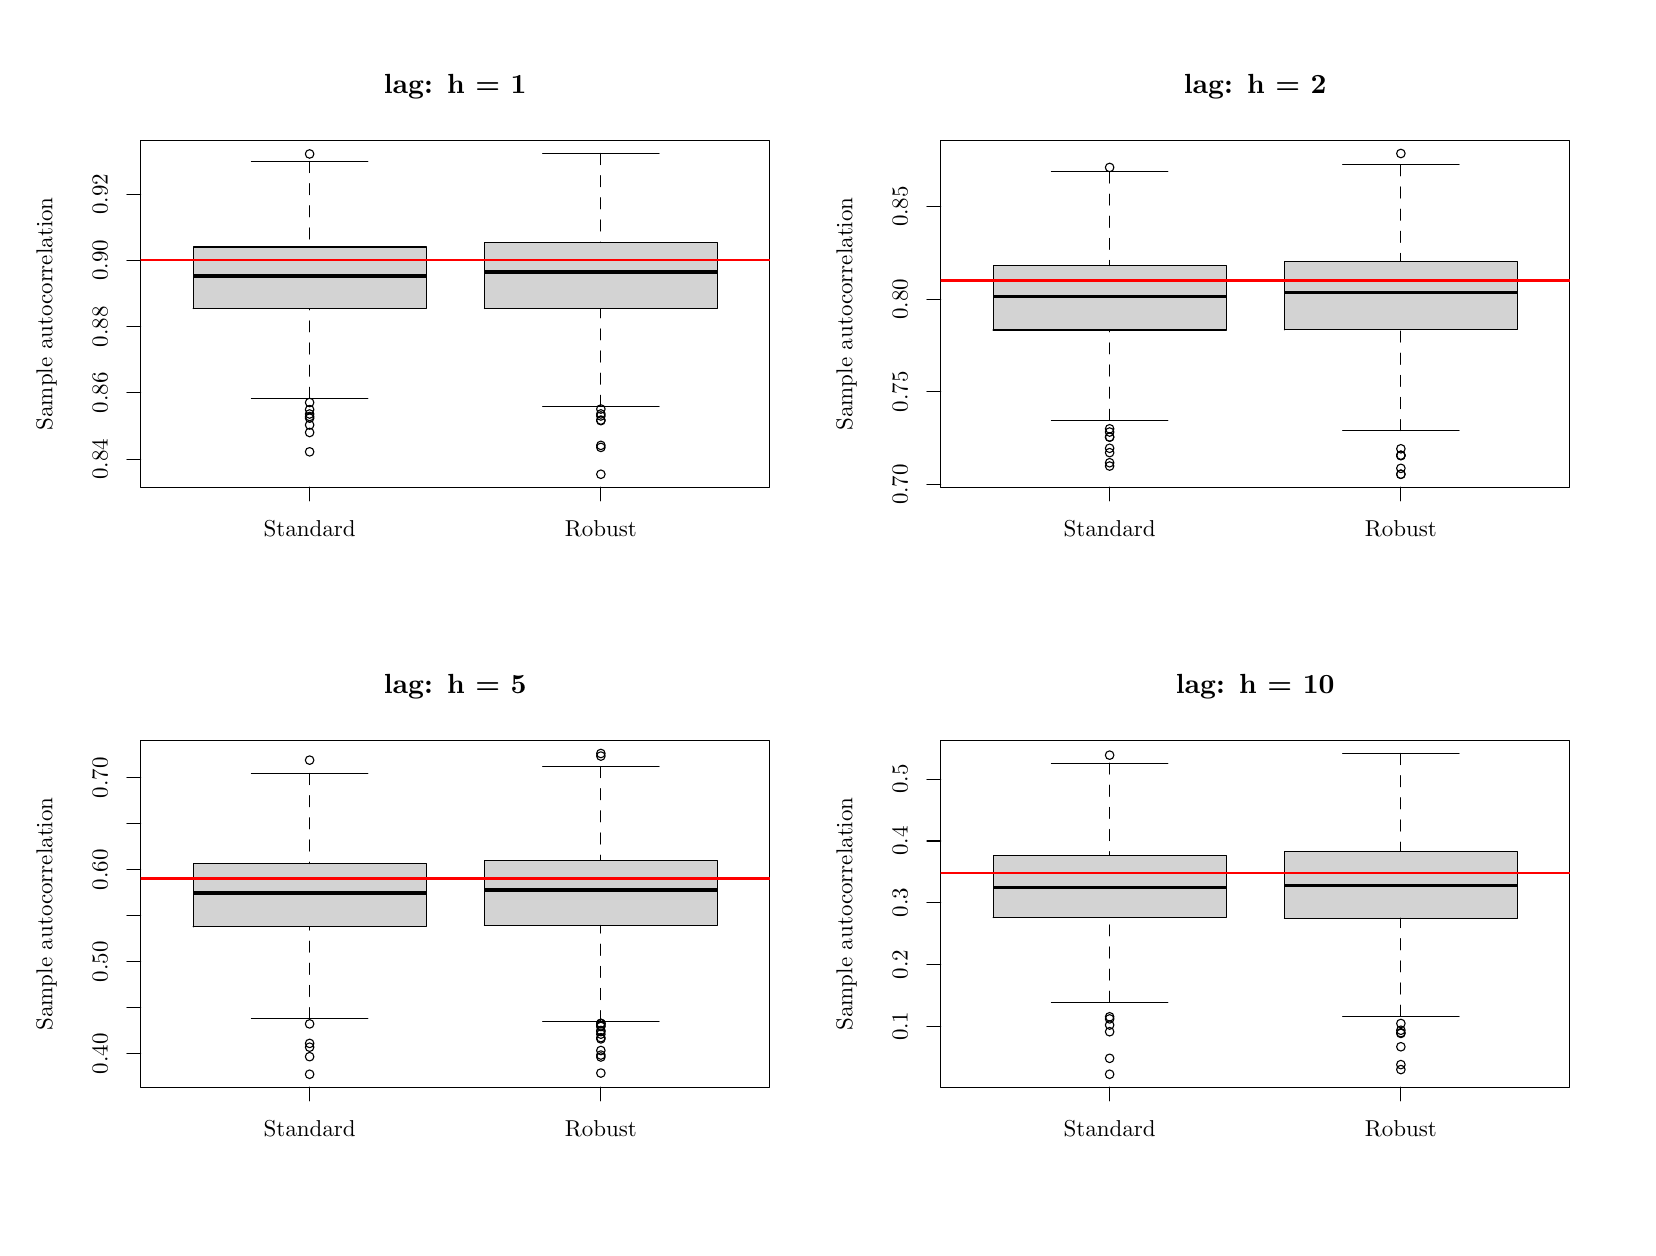
\begin{tikzpicture}[x=1pt,y=1pt]
\definecolor{fillColor}{RGB}{255,255,255}
\path[use as bounding box,fill=fillColor,fill opacity=0.00] (0,0) rectangle (578.16,433.62);
\begin{scope}
\path[clip] ( 40.84,267.61) rectangle (268.16,392.78);
\definecolor{fillColor}{RGB}{211,211,211}

\path[fill=fillColor] ( 59.78,332.10) --
	(143.98,332.10) --
	(143.98,354.35) --
	( 59.78,354.35) --
	cycle;
\definecolor{drawColor}{RGB}{0,0,0}

\path[draw=drawColor,line width= 1.2pt,line join=round] ( 59.78,343.91) -- (143.98,343.91);

\path[draw=drawColor,line width= 0.4pt,dash pattern=on 4pt off 4pt ,line join=round,line cap=round] (101.88,299.67) -- (101.88,332.10);

\path[draw=drawColor,line width= 0.4pt,dash pattern=on 4pt off 4pt ,line join=round,line cap=round] (101.88,385.26) -- (101.88,354.35);

\path[draw=drawColor,line width= 0.4pt,line join=round,line cap=round] ( 80.83,299.67) -- (122.93,299.67);

\path[draw=drawColor,line width= 0.4pt,line join=round,line cap=round] ( 80.83,385.26) -- (122.93,385.26);

\path[draw=drawColor,line width= 0.4pt,line join=round,line cap=round] ( 59.78,332.10) --
	(143.98,332.10) --
	(143.98,354.35) --
	( 59.78,354.35) --
	( 59.78,332.10);

\path[draw=drawColor,line width= 0.4pt,line join=round,line cap=round] (101.88,294.01) circle (  1.55);

\path[draw=drawColor,line width= 0.4pt,line join=round,line cap=round] (101.88,387.98) circle (  1.55);

\path[draw=drawColor,line width= 0.4pt,line join=round,line cap=round] (101.88,298.17) circle (  1.55);

\path[draw=drawColor,line width= 0.4pt,line join=round,line cap=round] (101.88,293.11) circle (  1.55);

\path[draw=drawColor,line width= 0.4pt,line join=round,line cap=round] (101.88,280.35) circle (  1.55);

\path[draw=drawColor,line width= 0.4pt,line join=round,line cap=round] (101.88,292.52) circle (  1.55);

\path[draw=drawColor,line width= 0.4pt,line join=round,line cap=round] (101.88,290.06) circle (  1.55);

\path[draw=drawColor,line width= 0.4pt,line join=round,line cap=round] (101.88,287.34) circle (  1.55);

\path[draw=drawColor,line width= 0.4pt,line join=round,line cap=round] (101.88,295.61) circle (  1.55);

\path[fill=fillColor] (165.02,332.08) --
	(249.22,332.08) --
	(249.22,356.07) --
	(165.02,356.07) --
	cycle;

\path[draw=drawColor,line width= 1.2pt,line join=round] (165.02,345.32) -- (249.22,345.32);

\path[draw=drawColor,line width= 0.4pt,dash pattern=on 4pt off 4pt ,line join=round,line cap=round] (207.12,296.78) -- (207.12,332.08);

\path[draw=drawColor,line width= 0.4pt,dash pattern=on 4pt off 4pt ,line join=round,line cap=round] (207.12,388.15) -- (207.12,356.07);

\path[draw=drawColor,line width= 0.4pt,line join=round,line cap=round] (186.07,296.78) -- (228.17,296.78);

\path[draw=drawColor,line width= 0.4pt,line join=round,line cap=round] (186.07,388.15) -- (228.17,388.15);

\path[draw=drawColor,line width= 0.4pt,line join=round,line cap=round] (165.02,332.08) --
	(249.22,332.08) --
	(249.22,356.07) --
	(165.02,356.07) --
	(165.02,332.08);

\path[draw=drawColor,line width= 0.4pt,line join=round,line cap=round] (207.12,295.81) circle (  1.55);

\path[draw=drawColor,line width= 0.4pt,line join=round,line cap=round] (207.12,294.03) circle (  1.55);

\path[draw=drawColor,line width= 0.4pt,line join=round,line cap=round] (207.12,291.82) circle (  1.55);

\path[draw=drawColor,line width= 0.4pt,line join=round,line cap=round] (207.12,293.31) circle (  1.55);

\path[draw=drawColor,line width= 0.4pt,line join=round,line cap=round] (207.12,272.24) circle (  1.55);

\path[draw=drawColor,line width= 0.4pt,line join=round,line cap=round] (207.12,282.68) circle (  1.55);

\path[draw=drawColor,line width= 0.4pt,line join=round,line cap=round] (207.12,281.95) circle (  1.55);

\path[draw=drawColor,line width= 0.4pt,line join=round,line cap=round] (207.12,291.61) circle (  1.55);
\end{scope}
\begin{scope}
\path[clip] (  0.00,  0.00) rectangle (578.16,433.62);
\definecolor{drawColor}{RGB}{0,0,0}

\path[draw=drawColor,line width= 0.4pt,line join=round,line cap=round] (101.88,267.61) -- (207.12,267.61);

\path[draw=drawColor,line width= 0.4pt,line join=round,line cap=round] (101.88,267.61) -- (101.88,262.63);

\path[draw=drawColor,line width= 0.4pt,line join=round,line cap=round] (207.12,267.61) -- (207.12,262.63);

\node[text=drawColor,anchor=base,inner sep=0pt, outer sep=0pt, scale=  0.83] at (101.88,249.68) {Standard};

\node[text=drawColor,anchor=base,inner sep=0pt, outer sep=0pt, scale=  0.83] at (207.12,249.68) {Robust};

\path[draw=drawColor,line width= 0.4pt,line join=round,line cap=round] ( 40.84,277.72) -- ( 40.84,373.46);

\path[draw=drawColor,line width= 0.4pt,line join=round,line cap=round] ( 40.84,277.72) -- ( 35.86,277.72);

\path[draw=drawColor,line width= 0.4pt,line join=round,line cap=round] ( 40.84,301.66) -- ( 35.86,301.66);

\path[draw=drawColor,line width= 0.4pt,line join=round,line cap=round] ( 40.84,325.59) -- ( 35.86,325.59);

\path[draw=drawColor,line width= 0.4pt,line join=round,line cap=round] ( 40.84,349.53) -- ( 35.86,349.53);

\path[draw=drawColor,line width= 0.4pt,line join=round,line cap=round] ( 40.84,373.46) -- ( 35.86,373.46);

\node[text=drawColor,rotate= 90.00,anchor=base,inner sep=0pt, outer sep=0pt, scale=  0.83] at ( 28.88,277.72) {0.84};

\node[text=drawColor,rotate= 90.00,anchor=base,inner sep=0pt, outer sep=0pt, scale=  0.83] at ( 28.88,301.66) {0.86};

\node[text=drawColor,rotate= 90.00,anchor=base,inner sep=0pt, outer sep=0pt, scale=  0.83] at ( 28.88,325.59) {0.88};

\node[text=drawColor,rotate= 90.00,anchor=base,inner sep=0pt, outer sep=0pt, scale=  0.83] at ( 28.88,349.53) {0.90};

\node[text=drawColor,rotate= 90.00,anchor=base,inner sep=0pt, outer sep=0pt, scale=  0.83] at ( 28.88,373.46) {0.92};
\end{scope}
\begin{scope}
\path[clip] (  0.00,216.81) rectangle (289.08,433.62);
\definecolor{drawColor}{RGB}{0,0,0}

\node[text=drawColor,anchor=base,inner sep=0pt, outer sep=0pt, scale=  1.00] at (154.50,409.77) {\bfseries lag: h =  1};

\node[text=drawColor,rotate= 90.00,anchor=base,inner sep=0pt, outer sep=0pt, scale=  0.83] at (  8.96,330.20) {Sample autocorrelation};
\end{scope}
\begin{scope}
\path[clip] (  0.00,  0.00) rectangle (578.16,433.62);
\definecolor{drawColor}{RGB}{0,0,0}

\path[draw=drawColor,line width= 0.4pt,line join=round,line cap=round] ( 40.84,267.61) --
	(268.16,267.61) --
	(268.16,392.78) --
	( 40.84,392.78) --
	( 40.84,267.61);
\end{scope}
\begin{scope}
\path[clip] ( 40.84,267.61) rectangle (268.16,392.78);
\definecolor{drawColor}{RGB}{255,0,0}

\path[draw=drawColor,line width= 0.8pt,line join=round,line cap=round] ( 40.84,349.53) -- (268.16,349.53);
\end{scope}
\begin{scope}
\path[clip] (329.92,267.61) rectangle (557.24,392.78);
\definecolor{fillColor}{RGB}{211,211,211}

\path[fill=fillColor] (348.86,324.38) --
	(433.06,324.38) --
	(433.06,347.63) --
	(348.86,347.63) --
	cycle;
\definecolor{drawColor}{RGB}{0,0,0}

\path[draw=drawColor,line width= 1.2pt,line join=round] (348.86,336.58) -- (433.06,336.58);

\path[draw=drawColor,line width= 0.4pt,dash pattern=on 4pt off 4pt ,line join=round,line cap=round] (390.96,291.72) -- (390.96,324.38);

\path[draw=drawColor,line width= 0.4pt,dash pattern=on 4pt off 4pt ,line join=round,line cap=round] (390.96,381.49) -- (390.96,347.63);

\path[draw=drawColor,line width= 0.4pt,line join=round,line cap=round] (369.91,291.72) -- (412.01,291.72);

\path[draw=drawColor,line width= 0.4pt,line join=round,line cap=round] (369.91,381.49) -- (412.01,381.49);

\path[draw=drawColor,line width= 0.4pt,line join=round,line cap=round] (348.86,324.38) --
	(433.06,324.38) --
	(433.06,347.63) --
	(348.86,347.63) --
	(348.86,324.38);

\path[draw=drawColor,line width= 0.4pt,line join=round,line cap=round] (390.96,288.67) circle (  1.55);

\path[draw=drawColor,line width= 0.4pt,line join=round,line cap=round] (390.96,287.50) circle (  1.55);

\path[draw=drawColor,line width= 0.4pt,line join=round,line cap=round] (390.96,275.21) circle (  1.55);

\path[draw=drawColor,line width= 0.4pt,line join=round,line cap=round] (390.96,285.72) circle (  1.55);

\path[draw=drawColor,line width= 0.4pt,line join=round,line cap=round] (390.96,276.41) circle (  1.55);

\path[draw=drawColor,line width= 0.4pt,line join=round,line cap=round] (390.96,383.11) circle (  1.55);

\path[draw=drawColor,line width= 0.4pt,line join=round,line cap=round] (390.96,281.63) circle (  1.55);

\path[draw=drawColor,line width= 0.4pt,line join=round,line cap=round] (390.96,280.06) circle (  1.55);

\path[draw=drawColor,line width= 0.4pt,line join=round,line cap=round] (390.96,285.64) circle (  1.55);

\path[fill=fillColor] (454.10,324.40) --
	(538.30,324.40) --
	(538.30,349.21) --
	(454.10,349.21) --
	cycle;

\path[draw=drawColor,line width= 1.2pt,line join=round] (454.10,338.00) -- (538.30,338.00);

\path[draw=drawColor,line width= 0.4pt,dash pattern=on 4pt off 4pt ,line join=round,line cap=round] (496.20,287.99) -- (496.20,324.40);

\path[draw=drawColor,line width= 0.4pt,dash pattern=on 4pt off 4pt ,line join=round,line cap=round] (496.20,384.04) -- (496.20,349.21);

\path[draw=drawColor,line width= 0.4pt,line join=round,line cap=round] (475.15,287.99) -- (517.25,287.99);

\path[draw=drawColor,line width= 0.4pt,line join=round,line cap=round] (475.15,384.04) -- (517.25,384.04);

\path[draw=drawColor,line width= 0.4pt,line join=round,line cap=round] (454.10,324.40) --
	(538.30,324.40) --
	(538.30,349.21) --
	(454.10,349.21) --
	(454.10,324.40);

\path[draw=drawColor,line width= 0.4pt,line join=round,line cap=round] (496.20,388.15) circle (  1.55);

\path[draw=drawColor,line width= 0.4pt,line join=round,line cap=round] (496.20,279.07) circle (  1.55);

\path[draw=drawColor,line width= 0.4pt,line join=round,line cap=round] (496.20,279.11) circle (  1.55);

\path[draw=drawColor,line width= 0.4pt,line join=round,line cap=round] (496.20,274.38) circle (  1.55);

\path[draw=drawColor,line width= 0.4pt,line join=round,line cap=round] (496.20,272.25) circle (  1.55);

\path[draw=drawColor,line width= 0.4pt,line join=round,line cap=round] (496.20,272.24) circle (  1.55);

\path[draw=drawColor,line width= 0.4pt,line join=round,line cap=round] (496.20,278.96) circle (  1.55);

\path[draw=drawColor,line width= 0.4pt,line join=round,line cap=round] (496.20,281.45) circle (  1.55);
\end{scope}
\begin{scope}
\path[clip] (  0.00,  0.00) rectangle (578.16,433.62);
\definecolor{drawColor}{RGB}{0,0,0}

\path[draw=drawColor,line width= 0.4pt,line join=round,line cap=round] (390.96,267.61) -- (496.20,267.61);

\path[draw=drawColor,line width= 0.4pt,line join=round,line cap=round] (390.96,267.61) -- (390.96,262.63);

\path[draw=drawColor,line width= 0.4pt,line join=round,line cap=round] (496.20,267.61) -- (496.20,262.63);

\node[text=drawColor,anchor=base,inner sep=0pt, outer sep=0pt, scale=  0.83] at (390.96,249.68) {Standard};

\node[text=drawColor,anchor=base,inner sep=0pt, outer sep=0pt, scale=  0.83] at (496.20,249.68) {Robust};

\path[draw=drawColor,line width= 0.4pt,line join=round,line cap=round] (329.92,268.54) -- (329.92,369.01);

\path[draw=drawColor,line width= 0.4pt,line join=round,line cap=round] (329.92,268.54) -- (324.94,268.54);

\path[draw=drawColor,line width= 0.4pt,line join=round,line cap=round] (329.92,302.03) -- (324.94,302.03);

\path[draw=drawColor,line width= 0.4pt,line join=round,line cap=round] (329.92,335.52) -- (324.94,335.52);

\path[draw=drawColor,line width= 0.4pt,line join=round,line cap=round] (329.92,369.01) -- (324.94,369.01);

\node[text=drawColor,rotate= 90.00,anchor=base,inner sep=0pt, outer sep=0pt, scale=  0.83] at (317.96,268.54) {0.70};

\node[text=drawColor,rotate= 90.00,anchor=base,inner sep=0pt, outer sep=0pt, scale=  0.83] at (317.96,302.03) {0.75};

\node[text=drawColor,rotate= 90.00,anchor=base,inner sep=0pt, outer sep=0pt, scale=  0.83] at (317.96,335.52) {0.80};

\node[text=drawColor,rotate= 90.00,anchor=base,inner sep=0pt, outer sep=0pt, scale=  0.83] at (317.96,369.01) {0.85};
\end{scope}
\begin{scope}
\path[clip] (289.08,216.81) rectangle (578.16,433.62);
\definecolor{drawColor}{RGB}{0,0,0}

\node[text=drawColor,anchor=base,inner sep=0pt, outer sep=0pt, scale=  1.00] at (443.58,409.77) {\bfseries lag: h =  2};

\node[text=drawColor,rotate= 90.00,anchor=base,inner sep=0pt, outer sep=0pt, scale=  0.83] at (298.04,330.19) {Sample autocorrelation};
\end{scope}
\begin{scope}
\path[clip] (  0.00,  0.00) rectangle (578.16,433.62);
\definecolor{drawColor}{RGB}{0,0,0}

\path[draw=drawColor,line width= 0.4pt,line join=round,line cap=round] (329.92,267.61) --
	(557.24,267.61) --
	(557.24,392.78) --
	(329.92,392.78) --
	(329.92,267.61);
\end{scope}
\begin{scope}
\path[clip] (329.92,267.61) rectangle (557.24,392.78);
\definecolor{drawColor}{RGB}{255,0,0}

\path[draw=drawColor,line width= 0.8pt,line join=round,line cap=round] (329.92,342.22) -- (557.24,342.22);
\end{scope}
\begin{scope}
\path[clip] ( 40.84, 50.80) rectangle (268.16,175.97);
\definecolor{fillColor}{RGB}{211,211,211}

\path[fill=fillColor] ( 59.78,108.68) --
	(143.98,108.68) --
	(143.98,131.57) --
	( 59.78,131.57) --
	cycle;
\definecolor{drawColor}{RGB}{0,0,0}

\path[draw=drawColor,line width= 1.2pt,line join=round] ( 59.78,120.90) -- (143.98,120.90);

\path[draw=drawColor,line width= 0.4pt,dash pattern=on 4pt off 4pt ,line join=round,line cap=round] (101.88, 75.54) -- (101.88,108.68);

\path[draw=drawColor,line width= 0.4pt,dash pattern=on 4pt off 4pt ,line join=round,line cap=round] (101.88,164.11) -- (101.88,131.57);

\path[draw=drawColor,line width= 0.4pt,line join=round,line cap=round] ( 80.83, 75.54) -- (122.93, 75.54);

\path[draw=drawColor,line width= 0.4pt,line join=round,line cap=round] ( 80.83,164.11) -- (122.93,164.11);

\path[draw=drawColor,line width= 0.4pt,line join=round,line cap=round] ( 59.78,108.68) --
	(143.98,108.68) --
	(143.98,131.57) --
	( 59.78,131.57) --
	( 59.78,108.68);

\path[draw=drawColor,line width= 0.4pt,line join=round,line cap=round] (101.88, 55.43) circle (  1.55);

\path[draw=drawColor,line width= 0.4pt,line join=round,line cap=round] (101.88, 73.63) circle (  1.55);

\path[draw=drawColor,line width= 0.4pt,line join=round,line cap=round] (101.88,168.94) circle (  1.55);

\path[draw=drawColor,line width= 0.4pt,line join=round,line cap=round] (101.88, 65.22) circle (  1.55);

\path[draw=drawColor,line width= 0.4pt,line join=round,line cap=round] (101.88, 66.58) circle (  1.55);

\path[draw=drawColor,line width= 0.4pt,line join=round,line cap=round] (101.88, 61.79) circle (  1.55);

\path[fill=fillColor] (165.02,109.24) --
	(249.22,109.24) --
	(249.22,132.76) --
	(165.02,132.76) --
	cycle;

\path[draw=drawColor,line width= 1.2pt,line join=round] (165.02,121.98) -- (249.22,121.98);

\path[draw=drawColor,line width= 0.4pt,dash pattern=on 4pt off 4pt ,line join=round,line cap=round] (207.12, 74.43) -- (207.12,109.24);

\path[draw=drawColor,line width= 0.4pt,dash pattern=on 4pt off 4pt ,line join=round,line cap=round] (207.12,166.64) -- (207.12,132.76);

\path[draw=drawColor,line width= 0.4pt,line join=round,line cap=round] (186.07, 74.43) -- (228.17, 74.43);

\path[draw=drawColor,line width= 0.4pt,line join=round,line cap=round] (186.07,166.64) -- (228.17,166.64);

\path[draw=drawColor,line width= 0.4pt,line join=round,line cap=round] (165.02,109.24) --
	(249.22,109.24) --
	(249.22,132.76) --
	(165.02,132.76) --
	(165.02,109.24);

\path[draw=drawColor,line width= 0.4pt,line join=round,line cap=round] (207.12, 73.71) circle (  1.55);

\path[draw=drawColor,line width= 0.4pt,line join=round,line cap=round] (207.12, 71.24) circle (  1.55);

\path[draw=drawColor,line width= 0.4pt,line join=round,line cap=round] (207.12, 72.69) circle (  1.55);

\path[draw=drawColor,line width= 0.4pt,line join=round,line cap=round] (207.12, 68.65) circle (  1.55);

\path[draw=drawColor,line width= 0.4pt,line join=round,line cap=round] (207.12, 55.87) circle (  1.55);

\path[draw=drawColor,line width= 0.4pt,line join=round,line cap=round] (207.12,170.41) circle (  1.55);

\path[draw=drawColor,line width= 0.4pt,line join=round,line cap=round] (207.12, 68.21) circle (  1.55);

\path[draw=drawColor,line width= 0.4pt,line join=round,line cap=round] (207.12, 69.93) circle (  1.55);

\path[draw=drawColor,line width= 0.4pt,line join=round,line cap=round] (207.12, 73.79) circle (  1.55);

\path[draw=drawColor,line width= 0.4pt,line join=round,line cap=round] (207.12,171.34) circle (  1.55);

\path[draw=drawColor,line width= 0.4pt,line join=round,line cap=round] (207.12, 70.87) circle (  1.55);

\path[draw=drawColor,line width= 0.4pt,line join=round,line cap=round] (207.12, 62.37) circle (  1.55);

\path[draw=drawColor,line width= 0.4pt,line join=round,line cap=round] (207.12, 72.93) circle (  1.55);

\path[draw=drawColor,line width= 0.4pt,line join=round,line cap=round] (207.12, 73.81) circle (  1.55);

\path[draw=drawColor,line width= 0.4pt,line join=round,line cap=round] (207.12, 64.02) circle (  1.55);

\path[draw=drawColor,line width= 0.4pt,line join=round,line cap=round] (207.12, 61.67) circle (  1.55);
\end{scope}
\begin{scope}
\path[clip] (  0.00,  0.00) rectangle (578.16,433.62);
\definecolor{drawColor}{RGB}{0,0,0}

\path[draw=drawColor,line width= 0.4pt,line join=round,line cap=round] (101.88, 50.80) -- (207.12, 50.80);

\path[draw=drawColor,line width= 0.4pt,line join=round,line cap=round] (101.88, 50.80) -- (101.88, 45.82);

\path[draw=drawColor,line width= 0.4pt,line join=round,line cap=round] (207.12, 50.80) -- (207.12, 45.82);

\node[text=drawColor,anchor=base,inner sep=0pt, outer sep=0pt, scale=  0.83] at (101.88, 32.87) {Standard};

\node[text=drawColor,anchor=base,inner sep=0pt, outer sep=0pt, scale=  0.83] at (207.12, 32.87) {Robust};

\path[draw=drawColor,line width= 0.4pt,line join=round,line cap=round] ( 40.84, 62.86) -- ( 40.84,162.60);

\path[draw=drawColor,line width= 0.4pt,line join=round,line cap=round] ( 40.84, 62.86) -- ( 35.86, 62.86);

\path[draw=drawColor,line width= 0.4pt,line join=round,line cap=round] ( 40.84, 79.48) -- ( 35.86, 79.48);

\path[draw=drawColor,line width= 0.4pt,line join=round,line cap=round] ( 40.84, 96.11) -- ( 35.86, 96.11);

\path[draw=drawColor,line width= 0.4pt,line join=round,line cap=round] ( 40.84,112.73) -- ( 35.86,112.73);

\path[draw=drawColor,line width= 0.4pt,line join=round,line cap=round] ( 40.84,129.35) -- ( 35.86,129.35);

\path[draw=drawColor,line width= 0.4pt,line join=round,line cap=round] ( 40.84,145.98) -- ( 35.86,145.98);

\path[draw=drawColor,line width= 0.4pt,line join=round,line cap=round] ( 40.84,162.60) -- ( 35.86,162.60);

\node[text=drawColor,rotate= 90.00,anchor=base,inner sep=0pt, outer sep=0pt, scale=  0.83] at ( 28.88, 62.86) {0.40};

\node[text=drawColor,rotate= 90.00,anchor=base,inner sep=0pt, outer sep=0pt, scale=  0.83] at ( 28.88, 96.11) {0.50};

\node[text=drawColor,rotate= 90.00,anchor=base,inner sep=0pt, outer sep=0pt, scale=  0.83] at ( 28.88,129.35) {0.60};

\node[text=drawColor,rotate= 90.00,anchor=base,inner sep=0pt, outer sep=0pt, scale=  0.83] at ( 28.88,162.60) {0.70};
\end{scope}
\begin{scope}
\path[clip] (  0.00,  0.00) rectangle (289.08,216.81);
\definecolor{drawColor}{RGB}{0,0,0}

\node[text=drawColor,anchor=base,inner sep=0pt, outer sep=0pt, scale=  1.00] at (154.50,192.96) {\bfseries lag: h =  5};

\node[text=drawColor,rotate= 90.00,anchor=base,inner sep=0pt, outer sep=0pt, scale=  0.83] at (  8.96,113.38) {Sample autocorrelation};
\end{scope}
\begin{scope}
\path[clip] (  0.00,  0.00) rectangle (578.16,433.62);
\definecolor{drawColor}{RGB}{0,0,0}

\path[draw=drawColor,line width= 0.4pt,line join=round,line cap=round] ( 40.84, 50.80) --
	(268.16, 50.80) --
	(268.16,175.97) --
	( 40.84,175.97) --
	( 40.84, 50.80);
\end{scope}
\begin{scope}
\path[clip] ( 40.84, 50.80) rectangle (268.16,175.97);
\definecolor{drawColor}{RGB}{255,0,0}

\path[draw=drawColor,line width= 0.8pt,line join=round,line cap=round] ( 40.84,126.19) -- (268.16,126.19);
\end{scope}
\begin{scope}
\path[clip] (329.92, 50.80) rectangle (557.24,175.97);
\definecolor{fillColor}{RGB}{211,211,211}

\path[fill=fillColor] (348.86,112.03) --
	(433.06,112.03) --
	(433.06,134.55) --
	(348.86,134.55) --
	cycle;
\definecolor{drawColor}{RGB}{0,0,0}

\path[draw=drawColor,line width= 1.2pt,line join=round] (348.86,122.82) -- (433.06,122.82);

\path[draw=drawColor,line width= 0.4pt,dash pattern=on 4pt off 4pt ,line join=round,line cap=round] (390.96, 81.44) -- (390.96,112.03);

\path[draw=drawColor,line width= 0.4pt,dash pattern=on 4pt off 4pt ,line join=round,line cap=round] (390.96,167.87) -- (390.96,134.55);

\path[draw=drawColor,line width= 0.4pt,line join=round,line cap=round] (369.91, 81.44) -- (412.01, 81.44);

\path[draw=drawColor,line width= 0.4pt,line join=round,line cap=round] (369.91,167.87) -- (412.01,167.87);

\path[draw=drawColor,line width= 0.4pt,line join=round,line cap=round] (348.86,112.03) --
	(433.06,112.03) --
	(433.06,134.55) --
	(348.86,134.55) --
	(348.86,112.03);

\path[draw=drawColor,line width= 0.4pt,line join=round,line cap=round] (390.96, 70.81) circle (  1.55);

\path[draw=drawColor,line width= 0.4pt,line join=round,line cap=round] (390.96, 61.19) circle (  1.55);

\path[draw=drawColor,line width= 0.4pt,line join=round,line cap=round] (390.96,170.74) circle (  1.55);

\path[draw=drawColor,line width= 0.4pt,line join=round,line cap=round] (390.96, 75.44) circle (  1.55);

\path[draw=drawColor,line width= 0.4pt,line join=round,line cap=round] (390.96, 55.43) circle (  1.55);

\path[draw=drawColor,line width= 0.4pt,line join=round,line cap=round] (390.96, 73.22) circle (  1.55);

\path[draw=drawColor,line width= 0.4pt,line join=round,line cap=round] (390.96, 76.20) circle (  1.55);

\path[fill=fillColor] (454.10,111.81) --
	(538.30,111.81) --
	(538.30,135.99) --
	(454.10,135.99) --
	cycle;

\path[draw=drawColor,line width= 1.2pt,line join=round] (454.10,123.63) -- (538.30,123.63);

\path[draw=drawColor,line width= 0.4pt,dash pattern=on 4pt off 4pt ,line join=round,line cap=round] (496.20, 76.43) -- (496.20,111.81);

\path[draw=drawColor,line width= 0.4pt,dash pattern=on 4pt off 4pt ,line join=round,line cap=round] (496.20,171.34) -- (496.20,135.99);

\path[draw=drawColor,line width= 0.4pt,line join=round,line cap=round] (475.15, 76.43) -- (517.25, 76.43);

\path[draw=drawColor,line width= 0.4pt,line join=round,line cap=round] (475.15,171.34) -- (517.25,171.34);

\path[draw=drawColor,line width= 0.4pt,line join=round,line cap=round] (454.10,111.81) --
	(538.30,111.81) --
	(538.30,135.99) --
	(454.10,135.99) --
	(454.10,111.81);

\path[draw=drawColor,line width= 0.4pt,line join=round,line cap=round] (496.20, 70.45) circle (  1.55);

\path[draw=drawColor,line width= 0.4pt,line join=round,line cap=round] (496.20, 57.13) circle (  1.55);

\path[draw=drawColor,line width= 0.4pt,line join=round,line cap=round] (496.20, 70.19) circle (  1.55);

\path[draw=drawColor,line width= 0.4pt,line join=round,line cap=round] (496.20, 73.78) circle (  1.55);

\path[draw=drawColor,line width= 0.4pt,line join=round,line cap=round] (496.20, 58.92) circle (  1.55);

\path[draw=drawColor,line width= 0.4pt,line join=round,line cap=round] (496.20, 71.34) circle (  1.55);

\path[draw=drawColor,line width= 0.4pt,line join=round,line cap=round] (496.20, 65.37) circle (  1.55);
\end{scope}
\begin{scope}
\path[clip] (  0.00,  0.00) rectangle (578.16,433.62);
\definecolor{drawColor}{RGB}{0,0,0}

\path[draw=drawColor,line width= 0.4pt,line join=round,line cap=round] (390.96, 50.80) -- (496.20, 50.80);

\path[draw=drawColor,line width= 0.4pt,line join=round,line cap=round] (390.96, 50.80) -- (390.96, 45.82);

\path[draw=drawColor,line width= 0.4pt,line join=round,line cap=round] (496.20, 50.80) -- (496.20, 45.82);

\node[text=drawColor,anchor=base,inner sep=0pt, outer sep=0pt, scale=  0.83] at (390.96, 32.87) {Standard};

\node[text=drawColor,anchor=base,inner sep=0pt, outer sep=0pt, scale=  0.83] at (496.20, 32.87) {Robust};

\path[draw=drawColor,line width= 0.4pt,line join=round,line cap=round] (329.92, 72.78) -- (329.92,162.06);

\path[draw=drawColor,line width= 0.4pt,line join=round,line cap=round] (329.92, 72.78) -- (324.94, 72.78);

\path[draw=drawColor,line width= 0.4pt,line join=round,line cap=round] (329.92, 95.10) -- (324.94, 95.10);

\path[draw=drawColor,line width= 0.4pt,line join=round,line cap=round] (329.92,117.42) -- (324.94,117.42);

\path[draw=drawColor,line width= 0.4pt,line join=round,line cap=round] (329.92,139.74) -- (324.94,139.74);

\path[draw=drawColor,line width= 0.4pt,line join=round,line cap=round] (329.92,162.06) -- (324.94,162.06);

\node[text=drawColor,rotate= 90.00,anchor=base,inner sep=0pt, outer sep=0pt, scale=  0.83] at (317.96, 72.78) {0.1};

\node[text=drawColor,rotate= 90.00,anchor=base,inner sep=0pt, outer sep=0pt, scale=  0.83] at (317.96, 95.10) {0.2};

\node[text=drawColor,rotate= 90.00,anchor=base,inner sep=0pt, outer sep=0pt, scale=  0.83] at (317.96,117.42) {0.3};

\node[text=drawColor,rotate= 90.00,anchor=base,inner sep=0pt, outer sep=0pt, scale=  0.83] at (317.96,139.74) {0.4};

\node[text=drawColor,rotate= 90.00,anchor=base,inner sep=0pt, outer sep=0pt, scale=  0.83] at (317.96,162.06) {0.5};
\end{scope}
\begin{scope}
\path[clip] (289.08,  0.00) rectangle (578.16,216.81);
\definecolor{drawColor}{RGB}{0,0,0}

\node[text=drawColor,anchor=base,inner sep=0pt, outer sep=0pt, scale=  1.00] at (443.58,192.96) {\bfseries lag: h =  10};

\node[text=drawColor,rotate= 90.00,anchor=base,inner sep=0pt, outer sep=0pt, scale=  0.83] at (298.04,113.38) {Sample autocorrelation};
\end{scope}
\begin{scope}
\path[clip] (  0.00,  0.00) rectangle (578.16,433.62);
\definecolor{drawColor}{RGB}{0,0,0}

\path[draw=drawColor,line width= 0.4pt,line join=round,line cap=round] (329.92, 50.80) --
	(557.24, 50.80) --
	(557.24,175.97) --
	(329.92,175.97) --
	(329.92, 50.80);
\end{scope}
\begin{scope}
\path[clip] (329.92, 50.80) rectangle (557.24,175.97);
\definecolor{drawColor}{RGB}{255,0,0}

\path[draw=drawColor,line width= 0.8pt,line join=round,line cap=round] (329.92,128.29) -- (557.24,128.29);
\end{scope}
\end{tikzpicture}
